\documentclass{article}
\usepackage{tabu}
\usepackage{amsmath}
\usepackage{algorithm2e}
\usepackage{graphicx}
\usepackage{comment}
%matrix environmentredef
\makeatletter
\renewcommand*\env@matrix[1][*\c@MaxMatrixCols c]{%
  \hskip -\arraycolsep
  \let\@ifnextchar\new@ifnextchar
  \array{#1}}

\renewenvironment{bmatrix}
{{\ifnum`}=0 \fi\left[\env@matrix}
{\endmatrix\right]\ifnum`{=0 \fi}}
\makeatother

\begin{document}

\title{CS 260: Homework 6}
\author{Daniel Lopez}
\maketitle

\date{11 August 2017}

\section{1}
\[
M=
	\begin{bmatrix}
	. & a & b & c & d & e & f \\
	a & X & 3 & X & 4 & X & 5 \\
	b & X & X & 1 & X & X & 1 \\
	c & X & X & X & 2 & X & X \\
	d & X & 3 & X & X & X & X \\
	e & X & X & X & 3 & X & 2 \\
	f & X & X & X & 2 & X & X
	\end{bmatrix}
\]
\section{2}

The tasks t1, t2, t3...tn can be run in parallel. If not, then the run time is the sum of t1 + t2 + t3 + ... + tn. If run in parallel, then the run time is that of the task with the longest execution time. In parallel, the run time will be O(tn) where tn is the longest execution time out of all of the tasks. 
\begin{comment}
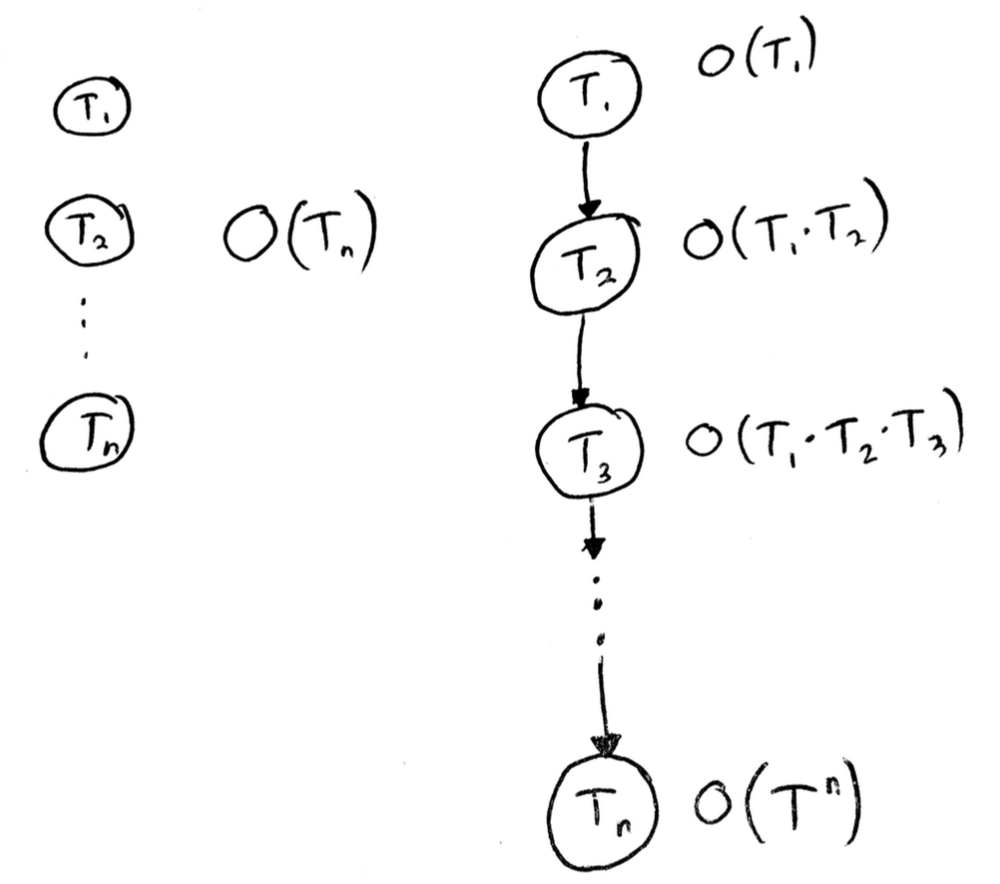
\includegraphics[scale=0.5]{graph2.jpg}
\end{comment}
\section{3}
Strong components: b, f, d, b-c-d
\section{4}
\begin{algorithm}
	\KwData{Insert edges}
	\mbox{Insert edge between vertex i and j.}
	Function Insert (i,j)
	\eIf {$i>n or j>n$}{
		PRINT Edge is not between i and j
	}{
	insert i at the end of i
	insert j at the end of j
	}
\end{algorithm}


\begin{algorithm}
	\KwData{Delete edges}
	\mbox{Delete edge between vertex i and j.}
	Function Delete (i,j)
	\eIf {$i>n or j>n$}{
		PRINT Edge is not between i and j
	}{
	Delete i at the end of i
	Delete j at the end of j
	}
\end{algorithm}


\newpage


\section{1 How to make tables}
\begin {center}
	\begin{tabular}{| c || c | c |}
	\hline
	1 & 2 & 3 \\ \hline
	7 & 8 & 9 \\ \hline
	12 & 13 & 14 \\ \hline
	\end{tabular}
\end{center}
\end{document}
